%%%%%%%%%%%%%%%%%%%%%%%%%%%%%%%%%%%%%%%%%%%%%%%%%%%%%%%%%%%%%%%%%%%%%
%%                                                                 %%
%% Please do not use \input{...} to include other tex files.       %%
%% Submit your LaTeX manuscript as one .tex document.              %%
%%                                                                 %%
%% All additional figures and files should be attached             %%
%% separately and not embedded in the \TeX\ document itself.       %%
%%                                                                 %%
%%%%%%%%%%%%%%%%%%%%%%%%%%%%%%%%%%%%%%%%%%%%%%%%%%%%%%%%%%%%%%%%%%%%%

%%\documentclass[referee,sn-basic]{sn-jnl}% referee option is meant for double line spacing

%%=======================================================%%
%% to print line numbers in the margin use lineno option %%
%%=======================================================%%

%%\documentclass[lineno,sn-basic]{sn-jnl}% Basic Springer Nature Reference Style/Chemistry Reference Style

%%======================================================%%
%% to compile with pdflatex/xelatex use pdflatex option %%
%%======================================================%%

%%\documentclass[pdflatex,sn-basic]{sn-jnl}% Basic Springer Nature Reference Style/Chemistry Reference Style

%%\documentclass[sn-basic]{sn-jnl}% Basic Springer Nature Reference Style/Chemistry Reference Style
\documentclass[sn-mathphys]{sn-jnl}% Math and Physical Sciences Reference Style
%%\documentclass[sn-aps]{sn-jnl}% American Physical Society (APS) Reference Style
%%\documentclass[sn-vancouver]{sn-jnl}% Vancouver Reference Style
%%\documentclass[sn-apa]{sn-jnl}% APA Reference Style
%%\documentclass[sn-chicago]{sn-jnl}% Chicago-based Humanities Reference Style
%%\documentclass[sn-standardnature]{sn-jnl}% Standard Nature Portfolio Reference Style
%%\documentclass[default]{sn-jnl}% Default
%%\documentclass[default,iicol]{sn-jnl}% Default with double column layout

%%%% Standard Packages
%%<additional latex packages if required can be included here>
%%%%

%%%%%=============================================================================%%%%
%%%%  Remarks: This template is provided to aid authors with the preparation
%%%%  of original research articles intended for submission to journals published
%%%%  by Springer Nature. The guidance has been prepared in partnership with
%%%%  production teams to conform to Springer Nature technical requirements.
%%%%  Editorial and presentation requirements differ among journal portfolios and
%%%%  research disciplines. You may find sections in this template are irrelevant
%%%%  to your work and are empowered to omit any such section if allowed by the
%%%%  journal you intend to submit to. The submission guidelines and policies
%%%%  of the journal take precedence. A detailed User Manual is available in the
%%%%  template package for technical guidance.
%%%%%=============================================================================%%%%
\usepackage{caption}

\jyear{2022}%

%% as per the requirement new theorem styles can be included as shown below
\theoremstyle{thmstyleone}%
%%\newtheorem{theorem}{Theorem}%  meant for continuous numbers
\newtheorem{theorem}{Theorem}[section]% meant for sectionwise numbers
%% optional argument [theorem] produces theorem numbering sequence instead of independent numbers for Proposition
\newtheorem{proposition}[theorem]{Proposition}%
%%\newtheorem{proposition}{Proposition}% to get separate numbers for theorem and proposition etc.

\theoremstyle{thmstyletwo}%
\newtheorem{example}{Example}%
\newtheorem{remark}{Remark}%

\theoremstyle{thmstylethree}%
\newtheorem{definition}{Definition}%

\newcommand{\CC}{\mathbb{C}}
\newcommand{\NN}{\mathbb{N}}
\newcommand{\QQ}{\mathbb{Q}}
\newcommand{\RR}{\mathbb{R}}
\newcommand{\ZZ}{\mathbb{Z}}

\newcommand{\eps}{\varepsilon}

\raggedbottom
%%\unnumbered% uncomment this for unnumbered level heads

\begin{document}

\title[Induction of Survival Trees by Quadric Splits and Dipolar Splitting Criteria]{Induction of Survival Trees by Quadric Splits and Dipolar Splitting Criteria}

%%=============================================================%%
%% Prefix	-> \pfx{Dr}
%% GivenName	-> \fnm{Joergen W.}
%% Particle	-> \spfx{van der} -> surname prefix
%% FamilyName	-> \sur{Ploeg}
%% Suffix	-> \sfx{IV}
%% NatureName	-> \tanm{Poet Laureate} -> Title after name
%% Degrees	-> \dgr{MSc, PhD}
%% \author*[1,2]{\pfx{Dr} \fnm{Joergen W.} \spfx{van der} \sur{Ploeg} \sfx{IV} \tanm{Poet Laureate}
%%                 \dgr{MSc, PhD}}\email{iauthor@gmail.com}
%%=============================================================%%

\author*[1,1]{\fnm{Aye Aye} \sur{Maung}}\email{a0maun01@louisville.edu}

\author[2,2]{\fnm{Drew} \sur{Lazar}}\email{dmlazar@bsu.edu}


\affil*[1]{\orgdiv{ Bioinformatics \& Biostatistics}, \orgname{University of Louisville}, \orgaddress{\street{485 E. Gray St.}, \city{Louisville}, \postcode{40202}, \state{KY}, \country{USA}}}

\affil[2]{\orgdiv{Mathematical Sciences}, \orgname{Ball State University}, \orgaddress{\street{Robert Bell Building, Room 465}, \city{Muncie}, \postcode{47306}, \state{IN}, \country{USA}}}

%%==================================%%
%% sample for unstructured abstract %%
%%==================================%%

\abstract{
In recent decades, a variety of statistical models and supervised learning algorithms have been extended to predict survival outcomes. In particular, classification and regression trees (CART) have been modified to account for right-censored survival data.  As in CART, sample data can be split univariately by considering covariates one at a time, obliquely with hyperplanes or non-linearly with curved surfaces. In this paper, we consider an existing non-parametric method which implements oblique splits and uses criteria based on pairs of covariates, and we extend this method to splits by quadratic surfaces. Data augmentation and optimization of combinations of piecewise-linear functions are used to find optimal quadric splits. Survival trees based on univariate splits and the log-rank statistic are also implemented. We compare the structure and predictive power of survival trees created by such trees on real and simulated data sets.}



\keywords{survival analysis, regression trees, non-linear trees, right-censored data, dipolar criteria, non-parametric statistics}

%%================================%%
%% Sample for structured abstract %%
%%================================%%

% \abstract{\textbf{Purpose:} The abstract serves both as a general introduction to the topic and as a brief, non-technical summary of the main results and their implications. The abstract must not include subheadings (unless expressly permitted in the journal's Instructions to Authors), equations or citations. As a guide the abstract should not exceed 200 words. Most journals do not set a hard limit however authors are advised to check the author instructions for the journal they are submitting to.
%
% \textbf{Methods:} The abstract serves both as a general introduction to the topic and as a brief, non-technical summary of the main results and their implications. The abstract must not include subheadings (unless expressly permitted in the journal's Instructions to Authors), equations or citations. As a guide the abstract should not exceed 200 words. Most journals do not set a hard limit however authors are advised to check the author instructions for the journal they are submitting to.
%
% \textbf{Results:} The abstract serves both as a general introduction to the topic and as a brief, non-technical summary of the main results and their implications. The abstract must not include subheadings (unless expressly permitted in the journal's Instructions to Authors), equations or citations. As a guide the abstract should not exceed 200 words. Most journals do not set a hard limit however authors are advised to check the author instructions for the journal they are submitting to.
%
% \textbf{Conclusion:} The abstract serves both as a general introduction to the topic and as a brief, non-technical summary of the main results and their implications. The abstract must not include subheadings (unless expressly permitted in the journal's Instructions to Authors), equations or citations. As a guide the abstract should not exceed 200 words. Most journals do not set a hard limit however authors are advised to check the author instructions for the journal they are submitting to.}

%%\pacs[JEL Classification]{D8, H51}

%%\pacs[MSC Classification]{35A01, 65L10, 65L12, 65L20, 65L70}

\maketitle

\section{Introduction} \label{sec:intro}


Two seminal works are credited with forming the basis for the development of survival analysis in the 20th century. The first was the work of Kaplan and Meier \cite{kaplanmeier}, where they introduced the Kaplan-Meier estimates as a non-parametric method of estimating survival probabilities.  The second was the proportional hazard model of Cox \cite{cox}, a widely used semi-parametric method of estimating survival times assuming the proportional hazards assumption.  Many more models and approaches from statistics have been adapted to accommodate survival analysis which often involves the presence of censored observations~\cite{oakes2001biometrika}. Survival analysis, in turn, has found wide application in finance, epidemiology, and insurance among many others.

In the last 40 years, tree-based survival analysis methods, which provide interpretable predictions without requiring the strong assumptions of parametric modeling techniques, have been developed. The first such model was introduced in~\cite{ciampi} and further development was presented in~\cite{gordonolshen} splitting nodes to attain the smallest amount of inter-node variability as measured by the Wasserstein metric. From there, many types of survival trees, mostly differing in the splitting criteria, were developed. These include univariate splits based on the log-rank statistic in~\cite{leblanccrowley}, splits based on likelihood ratio statistic and the assumption of constant hazards of the exponential model~\cite{bou2011review}, and completely non-parametric, oblique splits by hyperplanes in~\cite{kretowska}, among many others. This paper focuses on the improvement and extension of the methods introduced in ~\cite{kretowska} to accommodate non-linear splits. 

%%  The oblique splits of \cite{kretowska} This extended a previous dipolar method due to \cite{bobrowskikretowski} for non-survival data. 


\section{Background}

\subsection{Survival Data}

We assume that $N$ observations, $(\mathbf{x}_i, t_i, \delta_i)_{i = 1}^N$, are sampled from a random triple $(\mathbf{X}, T, \Delta)$.  $\mathbf{X}$ is a $D$-dimensional random covariate vector,
\[
T = \min(T_0, C)
\]
where $T_0$ is a random variable indicating survival time, $C$ is a random variable indicating right-censoring time and $\Delta = I(T_0 < C)$ is a censoring indicator.

\subsection{Survival Dipolar Criterion}

In \cite{kretowska}, a non-parametric, tree-based method of separating the covariate space of right-censored data by hyperplanes was proposed which extended the approach of \cite{bobrowskikretowski} to survival analysis. In both works, it is necessary to classify pairs of covariate vectors
\[
\{ (\mathbf{x}_i, \mathbf{x}_j) \}_{ 1 \leq i < j \leq N }
\]
known as \textit{dipoles} according to their time-difference information. Roughly speaking the aim is to label dipoles with small time differences as \textit{pure} and to label dipoles with large time differences as \textit{mixed}. We use the approach of \cite{kretowska} where, a vector of pairwise time differences $\Delta T$ is constructed as follows:

%Dipoles $(\mathbf{x}_i, \mathbf{x}_j)$ with sufficiently close uncensored survival times $t_i, t_j$ are labeled \emph{pure}. Dipoles $(\mathbf{x}_i, \mathbf{x}_j)$ with sufficiently far survival times $t_i, t_j$ that appropriate to compare and sufficiently far are labeled \emph{mixed}.  Dipoles whose censorship information makes comparisons inappropriate or whose survival times are neither too far nor too close are labeled \emph{neither}.

\begin{enumerate}[(1)]
\item Initialize $\Delta T$ as the empty vector
\item For each pair of time-censorship tuples from $\big\{\big((t_i, \delta_i),(t_j, \delta_j)\big)\big\}_{1 \leq i < j \leq N}$ append $\lvert t_i - t_j \rvert$ to $\Delta T$ if $\delta_k = 1$, where $k = \arg\min(t_i, t_j)$
%\item For each pair $((t_i, \delta_i),(t_j, \delta_j))$ from $(\mathbf{x}_i, t_i, \delta_i)_{i = 1}^N$, where $i<j$, add $|t_i - t_j|$ to $\Delta T$ if any of the following holds:
%\begin{enumerate}[(i)]
%\item $\delta_i = \delta_j = 1$,
%\item $\delta_i = 0, \delta_j = 1 \text{ and } t_i > t_j$, or
%\item $\delta_i = 1, \delta_j = 0 \text{ and } t_j > t_i$.
%\end{enumerate}
\end{enumerate} Next reals $0 < \eta < \zeta < 1$ are fixed as lower and upper percentile cutoffs of $\Delta T$ for determining \emph{pure} and \emph{mixed} dipoles.  Letting $\lvert\Delta T\rvert = L $ the floored products $\lfloor \eta \cdot L \rfloor$ and $\lfloor \zeta \cdot L \rfloor$ approximate the $\eta$-th and $\zeta$-th quantiles of $\Delta T$. Finally the survival dipolar criterion for $\{ (\mathbf{x}_i, \mathbf{x}_j) \}_{  1 \leq i < j \leq N }$ is defined:
\begin{enumerate}[(1)]
	\item $(\mathbf{x}_i, \mathbf{x}_j)$ is \emph{pure} if $\delta_i = \delta_j = 1$ and $\lvert t_i - t_j \rvert < \Delta T_{(\lfloor \eta \cdot L \rfloor)}$
	\item $(\mathbf{x}_i, \mathbf{x}_j)$  is \emph{mixed} if $\lvert t_i - t_j \rvert \geq \Delta T_{(\lfloor \zeta \cdot L \rfloor)}$ and $\delta_k = 1$, where $k = \arg\min(t_i, t_j)$
	
%	\item  A dipole $(\mathbf{x}_i, \mathbf{x}_j)$  is \emph{mixed} if $|t_j - t_i| \geq \Delta T_{(\lfloor \zeta \cdot L \rfloor)}$ and if one of the following holds:
%\begin{enumerate}[(i)]
%	\item $\delta_i = \delta_j = 1$ or
%    \item  $\delta_i = 0, \delta_j = 1, t_j < t_i$ or
%    \item $\delta_i = 1, \delta_j = 0, t_i < t_j$
%\end{enumerate}
	\item All other $(\mathbf{x}_i, \mathbf{x}_j)$ are \emph{neither}
\end{enumerate}

\subsection{Piecewise-Linear Criterion Functions} \label{sec:PLCF}


With dipoles labeled \cite{kretowska} splits the covariate space at nodes by hyperplanes intended to split many mixed dipoles while splitting few pure dipoles. To achieve this \cite{kretowska} employs linear combinations of special piecewise-linear functions which are specified as follows.

We specify any hyperplane
\[
H(\mathbf{v}) = \big\{(x_1,\ldots,x_D)^T \in \RR^D ; \mathbf{v}^T\mathbf{z} = 0 \text{ where } \mathbf{z} = (1, x_1,\ldots,x_D)^T \big\}
\]
by its coefficient vector $\mathbf{v} = (-\theta, w_1, \ldots, w_D)^T \in \RR^{D + 1}$. The\textit{ augmented vector }of a covariate vector $\mathbf{x}_j$ is $\mathbf{z}_j = (1, \mathbf{x}_j^T)^T$ and the\textit{ augmented dipole} of a dipole $(\mathbf{x}_j, \mathbf{x}_k)$ is $(\mathbf{z}_j, \mathbf{z}_k)$.

Now consider the piecewise-linear functions $\varphi^+_j, \varphi^-_j : \RR^{D + 1} \to \RR$:
	\begin{align}
		\varphi^+_j(\mathbf{v}) = \max\{0, \eps_j - \mathbf{v}^T \mathbf{z}_j\}, \quad
		\varphi^-_j(\mathbf{v}) = \max\{0, \eps_j + \mathbf{v}^T \mathbf{z}_j\} \label{eqs:PLC}
	\end{align} For $\mathbf{x}_j=(x_{1, j},\ldots,x_{D, j} )^T$, $\mathbf{z}_j =  (1, \mathbf{x}_j^T)^T$, $\mathbf{w} = (w_1, \ldots, w_D)^T$, $\mathbf{v} = (-\theta, \mathbf{w}^T)^T$
\[
 \mathbf{v}^T \mathbf{z}_j = \lVert \mathbf{w} \rVert \lVert \mathbf{d}_j \rVert \text{sgn}(o_j)
  \]
  where $\mathbf{d}_j = \frac{\mathbf{v}^T \mathbf{z}_j}{\lVert \mathbf{w} \rVert^2} \mathbf{w}$ is the shortest vector from $H(\mathbf{v})$ to $\mathbf{x}_j$ and $o_j$ is $1$ if $\mathbf{x}_j$ is orientated ``above''  $H(\mathbf{v})$ in the direction of $\mathbf{w}$ and $o_j$ is $-1$ if  $\mathbf{x}_j$ is orientated ``below''  $H(\mathbf{v})$ in the opposite direction of $\mathbf{w}$. Thus the $\eps_j$'s are called \textit{margins} and following \cite{bobrowskikretowski} we assume that
	\begin{align}
	\eps_j = \eps \text{ uniformly for all } j = 1, \ldots, N \label{eqs:uniformmargins}
	\end{align} for some fixed $\eps > 0$.


The piecewise-linear functions $\varphi^+_j$ and $\varphi^-_j$ are shown in Figure~\ref{fig:1}.

\begin{figure}[h]
	\centering
        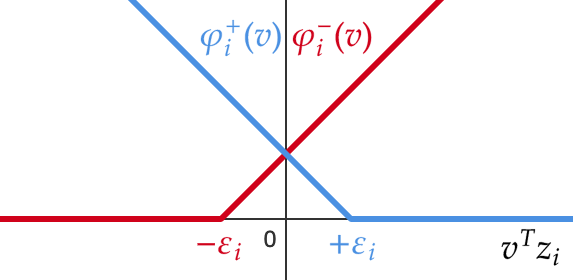
\includegraphics[height=.20\textwidth]{piecewiselinear}
        \caption{Piecewise-Linear Criterion Functions} \label{fig:1}
        \captionsetup{justification=centering}
%\vspace{15pt} 
%        \includegraphics[height=0.20\textwidth]{margins}
%        \caption{Margins of Piecewise Linear Functions} \label{fig:2}
      \end{figure}


\subsection{Dipole Penalty Functions} \label{sec:DPF}

Next \cite{kretowska} combines the functions in \eqref{eqs:PLC} to define two pairs of penalty functions. The pair of functions
\begin{align}
	\varphi^{m^+}_{jk} = \varphi^+_j + \varphi^-_k \text{ and } \varphi^{m^-}_{jk} = \varphi^-_j + \varphi^+_k  \label{eqs:mixedpenalty}
\end{align} penalize mixed dipoles that remain unsplit. Given a dipole $(\mathbf{x}_j, \mathbf{x}_k)$, each of these functions is minimized by a $\mathbf{v}$ which splits the dipole. On the other hand, the pair of functions
\begin{align}
	\varphi^{p^+}_{jk} = \varphi^+_j + \varphi^+_k \text{ and } \varphi^{p^-}_{jk} = \varphi^-_j + \varphi^-_k \label{eqs:purepenalty}
\end{align} penalize the splitting of pure dipoles. Given a dipole $(\mathbf{x}_j, \mathbf{x}_k)$, each of these functions is minimized by a $\mathbf{v}$ which does not split the dipole.


\subsection{Dipolar Criterion Functions} \label{sec:DCF}

Finally, using a weighted sum of penalty functions from~\eqref{eqs:mixedpenalty} and~\eqref{eqs:purepenalty}, \cite{kretowska} constructs an objective function that is minimized at a $\mathbf{v}$ for which many mixed dipoles are split and many pure dipoles are not split by $H(\mathbf{v})$. In optimizing the objective function, $\varphi^{m^+}_{jk}$ or $\varphi^{m^-}_{jk}$ from \eqref{eqs:mixedpenalty} are assigned to each mixed dipole and $\varphi^{p^+}_{jk}$ or $\varphi^{p^-}_{jk}$ from \eqref{eqs:purepenalty} are assigned to each pure dipole.

While \cite{kretowska} states assignments are made according to the ``orientation" of the dipoles, each dipole and its two elements do not intrinsically possess ``orientation'' without respect to a particular $\mathbf{v}$.   At the same time \cite{bobrowskikretowski} chooses $\varphi^{m^+}_{jk}$ for all mixed dipoles and chooses $\varphi^{p^+}_{jk}$ for all pure dipoles. In this paper, and as described in section~\ref{sec:OCDPF},  functions from \eqref{eqs:mixedpenalty} and \eqref{eqs:purepenalty} are assigned to dipoles in a geometrically reasonable manner with respect to initial $\mathbf{v}$'s at each step of the optimization algorithm and the dipolar criterion function is minimized with respect to those initial $\mathbf{v}$'s.

For now we introduce the dipolar criterion function presented in \cite{kretowska}. We can define dipoles as having ``positive orientation'' if  $\varphi^{m^+}_{jk}$ or $\varphi^{p^+}_{jk}$ are assigned to them and as having ``negative orientation'' if $\varphi^{m^-}_{jk}$ or $\varphi^{p^-}_{jk}$ are assigned to them. Following \cite{kretowska} let $I^{p^+}, I^{p^-}, I^{m^+}, I^{m^-}$ be the disjoint sets of pairs of indices of dipoles that are respectively: pure with positive orientation, pure with negative orientation, mixed with positive orientation and mixed with negative orientation. Then the dipolar criterion function is

\begin{align}
	\Psi = \sum_{\substack{(j, k) \\ \hspace{3.7pt} \in  I^{p^+}}} \alpha_{jk} \varphi^{p^+}_{jk} + \sum_{\substack{(j, k) \\ \hspace{3.7pt} \in I^{p^-}}} \alpha_{jk} \varphi^{p^-}_{jk} +\sum_{\substack{(j, k) \\ \hspace{3.7pt} \in I^{m^+}}} \alpha_{jk} \varphi^{m^+}_{jk} +\sum_{\substack{(j, k) \\ \hspace{3.7pt} \in I^{m^-}}} \alpha_{jk} \varphi^{m^-}_{jk} \label{eq:DPC_KRETOWSKA}
\end{align} The coefficients $\alpha_{jk} \geq 0$ are ``price'' factors of penalty functions. These can be fixed to prioritize splitting mixed dipoles or to prioritize not splitting pure dipoles depending on the relative sizes of the coefficients.

%% $\Psi$ is a nonnegative sum of piecewise-linear, convex functions. So it too is a piecewise-linear, convex function and can be minimized by convex optimization routines.


%\subsection{Dipolar Survival Trees}

\section{Methods}

\subsection{Orientation and Choice Dipole Penalty Functions} \label{sec:OCDPF}

In this section, we specify how we assign ``orientation'' to dipoles with respect to a given hyperplane $\mathbf{v}^\ast$. Functions from \eqref{eqs:mixedpenalty} are assigned to mixed dipoles and functions from \eqref{eqs:purepenalty} are assigned to pure dipoles with respect to a $\mathbf{v}^\ast$ based on these orientations. 

As in section~\ref{sec:PLCF}, let $\mathbf{v}^\ast$ be a coefficient vector and $(\mathbf{z}_j, \mathbf{z}_k)$ be an augmented dipole.
\begin{enumerate}[(1)]
	\item Let $(\mathbf{z}_j, \mathbf{z}_k)$ be pure. It has \emph{positive orientation} if ${\mathbf{v}^{\ast}}^T (\mathbf{z}_j + \mathbf{z}_k) \geq 0$ and in this case we assign $\varphi^{p^+}_{jk}$ to it. It has \emph{negative orientation} if ${{\mathbf{v}^\ast}}^T (\mathbf{z}_j + \mathbf{z}_k) \leq 0$ and in this case we assign $\varphi^{p^-}_{jk}$ to it.
	\item Let $(\mathbf{z}_j, \mathbf{z}_k)$ be mixed. It has a \emph{positive orientation} if ${\mathbf{v}^{\ast}}^T (\mathbf{z}_j - \mathbf{z}_k) \geq 0$ and in this case we assign $\varphi^{m^+}_{jk}$ to it. It has a \emph{negative orientation} if ${{\mathbf{v}^\ast}}^T (\mathbf{z}_j - \mathbf{z}_k) \leq 0$ and in this case we assign $\varphi^{m^-}_{jk}$ to it.
\end{enumerate}

The index sets of the dipole criterion function $\eqref{eq:DPC_KRETOWSKA}$ now depend on $\mathbf{v}^\ast$: $I^{p^+}_{\mathbf{v}^\ast}, I^{p^-}_{\mathbf{v}^\ast}, I^{m^+}_{\mathbf{v}^\ast}, I^{m^-}_{\mathbf{v}^\ast}$. In our algorithm to find a splitting hyperplane, we therefore optimize the function
\begin{align}
	\Psi_{\mathbf{v}^\ast} = \sum_{\substack{(j, k) \\ \hspace{3.7pt} \in   I^{p^+}_{\mathbf{v}^\ast}}} \alpha_{jk} \varphi^{p^+}_{jk} + \sum_{\substack{(j, k) \\ \hspace{3.7pt} \in  I^{p^-}_{\mathbf{v}^\ast}}} \alpha_{jk} \varphi^{p^-}_{jk} +\sum_{\substack{(j, k) \\  \hspace{3.7pt} \in I^{m^+}_{\mathbf{v}^\ast}}} \alpha_{jk} \varphi^{m^+}_{jk} +\sum_{\substack{(j, k)   \\ \hspace{3.7pt} \in I^{m^-}_{\mathbf{v}^\ast}}} \alpha_{jk} \varphi^{m^-}_{jk} \label{eq:DPC}
\end{align}

Below we justify our assignments of penalty functions based on orientation with respect to a particular $\mathbf{v}^\ast$.

\begin{proposition} \hfill
\begin{itemize}
	\item[(a)] If ${\mathbf{v}^{\ast}}^T (\mathbf{z}_j + \mathbf{z}_k) \geq 0$, then $\varphi^{p^-}_{jk}(\mathbf{v}^{\ast}) \geq \varphi^{p^+}_{jk}(\mathbf{v}^{\ast})$.
	\item[(b)] If ${\mathbf{v}^{\ast}}^T (\mathbf{z}_j + \mathbf{z}_k) \leq 0$, then $\varphi^{p^+}_{jk}(\mathbf{v}^{\ast}) \geq \varphi^{p^-}_{jk}(\mathbf{v}^{\ast})$.
	\item[(c)] If ${\mathbf{v}^{\ast}}^T (\mathbf{z}_j - \mathbf{z}_k) \geq 0$, then $\varphi^{m^-}_{jk}(\mathbf{v}^{\ast}) \geq \varphi^{m^+}_{jk}(\mathbf{v}^{\ast})$.
	\item[(d)] If ${\mathbf{v}^{\ast}}^T (\mathbf{z}_j - \mathbf{z}_k) \leq 0$, then $\varphi^{m^+}_{jk}(\mathbf{v}^{\ast}) \geq \varphi^{m^-}_{jk}(\mathbf{v}^{\ast})$.
\end{itemize}
\end{proposition}

\begin{proof} We show (a) with (b)-(d) shown similarly. Assuming $\eps_j = \eps_k = \eps$ as in \eqref{eqs:uniformmargins},
\begin{align*}
{\mathbf{v}^{\ast}}^T (\mathbf{z}_j + \mathbf{z}_k) \geq 0 &\implies \eps + {\mathbf{v}^{\ast}}^T \mathbf{z}_j + {\mathbf{v}^{\ast}}^T\mathbf{z}_k \geq \eps \\
 	&\implies \eps_j + {\mathbf{v}^{\ast}}^T \mathbf{z}_j \geq \eps_k - {\mathbf{v}^{\ast}}^T \mathbf{z}_k \text{ and } \eps_k + {\mathbf{v}^{\ast}}^T \mathbf{z}_k \geq \eps_j - {\mathbf{v}^{\ast}}^T \mathbf{z}_j
\end{align*} Thus
\begin{gather*}
\varphi^-_j(\mathbf{v}^{\ast}) = \max\{0, \eps_j + {\mathbf{v}^{\ast}}^T \mathbf{z}_j\} \geq \max\{0, \eps_k - {\mathbf{v}^{\ast}}^T \mathbf{z}_k\} = \varphi^+_k(\mathbf{v}^{\ast}) \\
\varphi^-_k(\mathbf{v}^{\ast}) = \max\{0, \eps_k + {\mathbf{v}^{\ast}}^T \mathbf{z}_k\} \geq \max\{0, \eps_j - {\mathbf{v}^{\ast}}^T \mathbf{z}_j\} = \varphi^+_j(\mathbf{v}^{\ast})
\end{gather*} implying that
$$
\varphi^{p^-}_{jk}(\mathbf{v}^{\ast}) = \varphi^-_j(\mathbf{v}^{\ast}) + \varphi^-_k(\mathbf{v}^{\ast}) \geq \varphi^+_k(\mathbf{v}^{\ast}) + \varphi^+_j(\mathbf{v}^{\ast}) = \varphi^+_j(\mathbf{v}^{\ast}) + \varphi^+_k(\mathbf{v}^{\ast}) = \varphi^{p^+}_{jk}(\mathbf{v}^{\ast})
$$
\end{proof}

The sizes of the penalties $\varphi^{p^+}_{jk}(\mathbf{v}^{\ast})$ and $\varphi^{p^-}_{jk}(\mathbf{v}^{\ast})$ for a pure positively-oriented dipole are shown in Figure~\ref{fig:2}. $\lVert \mathbf{w}^{\ast} \rVert = 1$ is assumed for simplicity.

\begin{figure}[h]
	\centering
        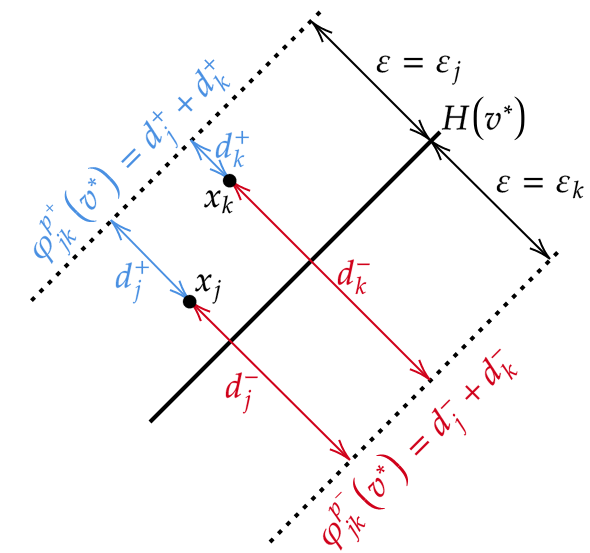
\includegraphics[height=.395\textwidth]{purepositivepenalties}
        \caption{Penalties for a Pure Positively-Oriented Dipole} \label{fig:2}
        \captionsetup{justification=centering}
%\vspace{15pt} 
%        \includegraphics[height=0.20\textwidth]{margins}
%        \caption{Margins of Piecewise Linear Functions} \label{fig:2}
      \end{figure} 
      
In other words choosing $\varphi^{p^+}_{jk}$ over $\varphi^{p^-}_{jk}$, for a pure positively oriented dipole, penalizes our guess of the splitting hyperplane $\mathbf{v}^{\ast}$ less. This is what we want if $\mathbf{v}^{\ast}$ was close to the optimal to begin with. Of course in general the preliminary guess $\mathbf{v}^{\ast}$ would not be optimal. In section~\ref{sec:ROA} we describe an algorithm to get rid of this dependence on a preliminary guess.


\subsection{Optimization of Dipolar Criterion Functions} 

\subsection{Re-Orientation Algorithm} \label{sec:ROA}

\subsection{Quadric Augmentation of Covariates}

\section{Data}



\section{Results}\label{sec2}

Sample body text. Sample body text. Sample body text. Sample body text. Sample body text. Sample body text. Sample body text. Sample body text.

\section{Conclusions} 

\section*{Declarations}

Some journals require declarations to be submitted in a standardised format. Please check the Instructions for Authors of the journal to which you are submitting to see if you need to complete this section. If yes, your manuscript must contain the following sections under the heading `Declarations':

\begin{itemize}
\item Funding
\item Conflict of interest/Competing interests (check journal-specific guidelines for which heading to use)
\item Ethics approval
\item Consent to participate
\item Consent for publication
\item Availability of data and materials
\item Code availability
\item Authors' contributions
\end{itemize}

\noindent
If any of the sections are not relevant to your manuscript, please include the heading and write `Not applicable' for that section.

%%===================================================%%
%% For presentation purpose, we have included        %%
%% \bigskip command. please ignore this.             %%
%%===================================================%%
\bigskip
\begin{flushleft}%
Editorial Policies for:

\bigskip\noindent
Springer journals and proceedings: \url{https://www.springer.com/gp/editorial-policies}

\bigskip\noindent
Nature Portfolio journals: \url{https://www.nature.com/nature-research/editorial-policies}

\bigskip\noindent
\textit{Scientific Reports}: \url{https://www.nature.com/srep/journal-policies/editorial-policies}

\bigskip\noindent
BMC journals: \url{https://www.biomedcentral.com/getpublished/editorial-policies}
\end{flushleft}

\begin{appendices}

\section{Section title of first appendix}\label{secA1}

An appendix contains supplementary information that is not an essential part of the text itself but which may be helpful in providing a more comprehensive understanding of the research problem or it is information that is too cumbersome to be included in the body of the paper.

%%=============================================%%
%% For submissions to Nature Portfolio Journals %%
%% please use the heading ``Extended Data''.   %%
%%=============================================%%

%%=============================================================%%
%% Sample for another appendix section			       %%
%%=============================================================%%

%% \section{Example of another appendix section}\label{secA2}%
%% Appendices may be used for helpful, supporting or essential material that would otherwise
%% clutter, break up or be distracting to the text. Appendices can consist of sections, figures,
%% tables and equations etc.

\end{appendices}

%%===========================================================================================%%
%% If you are submitting to one of the Nature Portfolio journals, using the eJP submission   %%
%% system, please include the references within the manuscript file itself. You may do this  %%
%% by copying the reference list from your .bbl file, paste it into the main manuscript .tex %%
%% file, and delete the associated \verb+\bibliography+ commands.                            %%
%%===========================================================================================%%

\bibliography{Sources}% common bib file
%% if required, the content of .bbl file can be included here once bbl is generated
%%\input sn-article.bbl
%% Default %%
%%\input sn-sample-bib.tex%

\end{document}
